\documentclass{article}
\usepackage{amsmath,amsfonts,amssymb,graphicx,fullpage}
\usepackage{mdframed}
\usepackage{multicol}
\usepackage{microtype}
\usepackage{hyperref}
\usepackage{csquotes}
\usepackage{hyperref}
\hypersetup{
    colorlinks=true,
    linkcolor=blue,
    filecolor=magenta,      
    urlcolor=cyan,
    pdftitle={Overleaf Example},
    pdfpagemode=FullScreen,
    }
    
\definecolor{quotemark}{gray}{0.7}
\makeatletter
\newlength\origparskip

\newcommand{\fquote}{%
  \@ifnextchar[{\fquote@i}{\fquote@i[]}%]
}

\def\fquote@i[#1]{%
  \@ifnextchar[{\fquote@ii{#1}}{\fquote@ii{#1}[]}%]
}%

\def\fquote@ii#1[#2]{%
  \def\pqm@tempa{#1}%
  \def\pqm@tempb{#2}%
  \noindent
  \list
    {}
    {\setlength{\leftmargin}{0.3\textwidth}%
     \setlength{\rightmargin}{0.1\textwidth}%
     \setlength{\origparskip}{\parskip}}%
    \item[]%
      \begin{picture}(0,0)%
        \put(-15,-8){\makebox(0,0){\scalebox{4}{%
          \textcolor{quotemark}{\textquotedblright}}}}%
      \end{picture}%
      \begingroup
      \itshape
      \ignorespaces}%

\def\endfquote{%
  \endgroup
  \par
  \raggedleft
  \ifx\pqm@tempa\empty
  \else
    {\bfseries --- \pqm@tempa\par}%
    \setlength{\parskip}{\origparskip}%
    \ifx\pqm@tempb\empty
    \else
      (\pqm@tempb)%
    \fi
  \fi
  \par
  \endlist}
\makeatother


\title{FunML: Fundamentals of Machine Learning}

\begin{document}

\maketitle

\begin{center}
{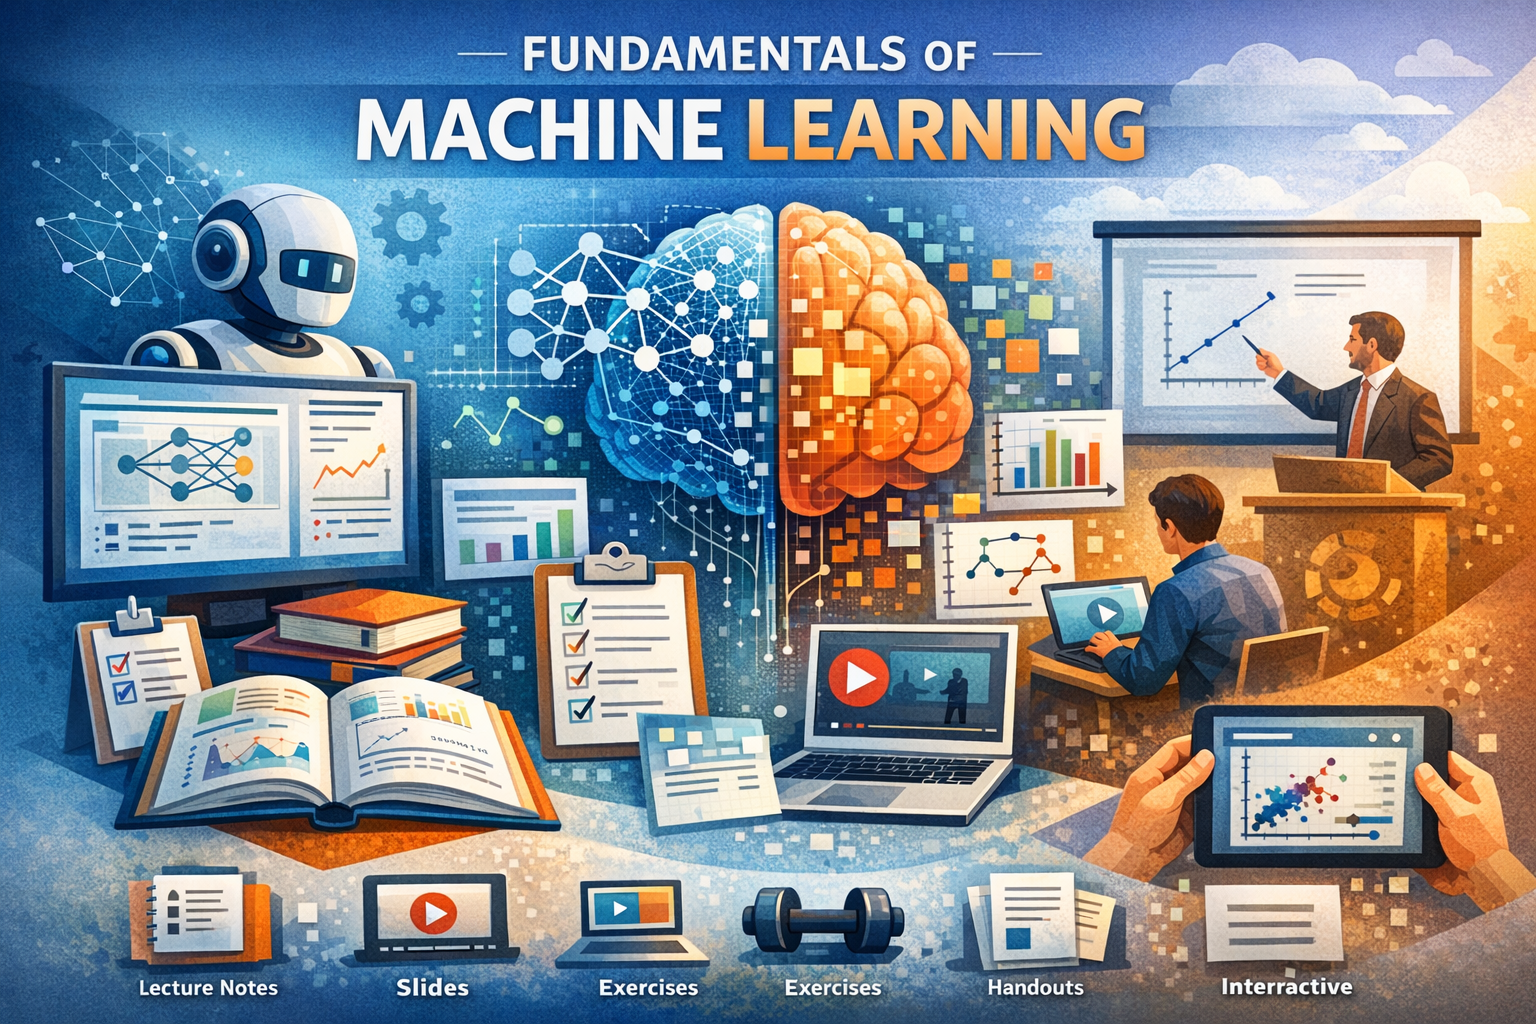
\includegraphics[width=0.9\linewidth]{img/Lecture0/ChatGPT Course Image.png}}
\end{center}

\section{Preface}

\begin{fquote}[Franklin D. Roosevelt][$32nd$ President of the United States of America]
    The test of our progress is not whether we add more to the abundance of those who have much, it is whether we provide enough for those who have little.
  \end{fquote}

This quote from Franklin D. Roosevelt (FDR) curiously captures the motivation behind designing good machine learning algorithms. Roosevelt was quoted saying this at his inaugural address on January 20, 1937. FDR's economic policies, titled the \emph{New Deal} were already in place. The above inaugural address rhetoric was directed towards strengthening and expanding the governmental programs to help US citizens who were struggling during the depression era of the 1930s. Machine learning (ML) deals with extracting meaningful information from a large corpus of data. Modern ML progress is often associated with \emph{large-scale} learning. This includes larger datasets, larger models, and greater computational resources. However, a more meaningful measure of progress is the ability to learn effectively from limited and noisy data that does not always conform to scale-driven learning. In many real-world settings, data is expensive, scarce, unfair, imbalanced, and impractical, or even immoral to obtain. Traditionally, ML research seeks to right this imbalance by constructing equitable and fair algorithms through better inductive biases, representation learning, or apriori knowledge. Hence, the central challenge of machine learning is not simply to extend the abundant but to equitably use the little data we have by constructing intelligent algorithms.    

\section{Vision}

ML and its applications in Artificial Intelligence (AI) have permeated everyday lives including healthcare, transport, education, energy, entertainment, and finance among others. People with no exposure to data science or engineering principles are aware of ML techniques. Industries use ML to attract customers, market and sell products, recruit for workplace, power software applications, improve efficiency and so on. The significant interest from everyday people and industries has ensured ML a permanent place in undergraduate and graduate curricula.  

The applicability of ML in multiple disciplines including electrical and computer engineering, computer science, civil engineering, industrial engineering, biomedical engineering, and mechanical engineering, among many other fields, has given rise to multiple cross-listed courses across the curricula. There are a diverse set of researchers from all the above disciplines, who bring their individuality to ML writing and education. As a growing interdisciplinary field, ML and specifically deep learning (DL) is susceptible to redefining terminologies. Oftentimes, this redefinition is a necessary evolution. However, for beginners learning ML, changing terminologies is a cause for confusion. For instance, the words ‘high-dimensional features’, ‘activations’, ‘embeddings’, ‘latent representation’ and ‘hidden representations’ all refer to the same concept under different contexts. It is necessary to separate ML-research with ML-education, while also keeping up with ML evolution. As such, the purpose of this book is to allow students with no or limited knowledge about data-driven techniques and engineering to comprehend ML theory and techniques as well as acquire the skills to deploy such systems on real data.

\section{Why this Book?}

ML is often introduced either as a toolbox of algorithms or as a sequence of mathematically dense topics. It is standard practice for introductory courses to linearly discuss regression, regularization, generalization, optimization, and inference. Such a regimented approach to learning does not translate well today since students have already been exposed to ML-driven AI tools from a young age. The book differs from existing works in the following ways:

\begin{itemize}
    \item Vision: From the start, the vision of the book is to cater to an audience that has a superficial (and possibly wildly incorrect) view of ML algorithms. It is designed to be a modular, and dynamic resource of education that can be continuously updated over time. The book is an integrated part of the crosslisted undergraduate and graduate level course on Fundamentals of Machine Learning course at Georgia Tech within the Electrical and Computer Engineering department. It is also crosslisted across other departments including \textcolor{red}{design engineering, computer science etc.} as an elective.
    \item Multimodal Learning: Apart from the explanatory content within the lecture notes, the book composes of lecture slides, exercises, lecture videos, demos, interactive notebooks, and handouts. The coupled nature of all these resources within each chapter ensures that the concepts are reinforced through multiple modalities.
    \item Module-based Learning: There are seven large modules. In sequence, these are classification, regression, clustering, convolutional neural networks, autoencoders, sequence models, and advanced topics. Each module generally follows the following structure: 
    \begin{itemize}
        \item Description of the problem that is tackled by the module in consideration along with real world examples and interactive demos.
        \item Foundational algorithms that tackle the problem along with interactive demos for the intuitions and the algorithms themselves, depending on compute requirements.
        \item Performance metrics that showcase tradeoffs between constraints and requirements within the problem setting.
    \end{itemize}
    The modules are designed to promote transferable understanding. Rather than focusing on individual algorithms in isolation, the book highlights recurring ideas including intuitions, algorithms, and performance metrics, across modules. This helps students adapt to new methods and evolving course content.
    \item Course structure: The book perfectly aligns with a university and college-level course structure with chapters divided into coherent lecture topics. The chapters are also modular to allow instructors to adapt the book based on semester-trimester-summer lengths, availability, coverage, and required depth.  
    \item Interactivity: Multiple interactive Jupyterlite notebooks are provided within each chapter to aid student learning experience. The intuition is derived from visually interacting with such tools from within your browser. The interactive nature makes abstract and difficult content accessible to students at all levels.
    \item ML for All: The book has been crafted to ensure minimum prerequisites. All students, irrespective of discipline, use ML models for a variety of reasons including to write code, retrieve information, design logos, and generally converse. Existing courses on ML focus on a `bottom-up' approach to modeling. These courses do not prepare students for understanding the utility of trained models. For instance, students cannot replicate their previous interactions with DALL-E even though they use the same prompts repeatedly because, they are unaware of the distributional sampling nature of Generative AI models. The book presents a practical view of ML and its utility.
    \item Caters to students and instructors: The book is explicitly designed to serve both students and instructors. Students receive layered explanations and interactive practice opportunities, while instructors gain a modular and ready-to-deploy teaching framework.
    \item Resource-aware: Assignments and exercises are designed keeping in mind the resource constraints of students. Hardware requirements include access to a computer with internet. Jupyterlite will be used extensively. 
\end{itemize}


\section{Target Audience}
The book is primarily targeted towards undergraduate and graduate students at universities with a basic background in linear algebra, probability, and statistics, as well as python programming. The book provides the necessary prerequisite details for using deep learning tools like Pytorch. Links to additional resources are provided wherever applicable. The chapters are designed with in-person lecture time constraints in mind. Additionally, practitioners who want to engage with a deeper understanding of machine learning will find the book relevant.

\section{Resources}
The book is a dynamic and multimodal resource of education for students and instructors. The book consisted of lecture notes and slides used in classrooms, links to lecture videos, exercises, and interactive notebooks whenever possible. The book has been designed to function both as a self-study resource for students and practitioners and as a complete teaching toolkit for instructors. The book provides the following resources:

\begin{itemize}
    \item Lecture Notes: Consists of the primary course material, with detailed explanations, mathematical notations, prerequisites and derivations, and key insights.
    \item Slides: Concise summaries for students and perfect in-class material for instructors. Students are encouraged to use the lecture notes and summaries together.
    \item Exercises: Problems designed to test and expand student learning. These problem sets consist of both conceptual and analytical questions. 
    \item Videos: Video lectures from the \emph{Fundamentals and Applications of Machine Learning Course} across multiple semesters and instructors from the Electrical and Computer Engineering Department at Georgia Institute of Technology.
    \item Demos and Interactive Notebooks: Interactive Jupyterlite notebooks that provide visual aids to understand abstract concepts within the notes. Students are encouraged to play around with demos to get an idea of such concepts. 
    \item Handouts: These are external resources for students to think and apply learned curriculum beyond course materials.
    \item Concept tags: A key feature, that utilizes its online nature, is concept tags. Concept tags allow instructors to construct their own curricula geared towards graduate, or lower-level and upper-level undergraduate students. Concept tags connect similar concepts between disparate lectures. For instance, regularization is currently introduced in chapter 8 within regression, after discussion of classification algorithms and performance metrics. Instructors interested in discussion of regularization can use concept tags to draw materials from different lectures.
\end{itemize}

\section{How to Use this Book?}

The resources in this book caters to both students and educators.

\begin{itemize}
    \item For students: We recommend utilizing the slides and notes in conjunction for a complete understanding of the materials. The notes go into detail regarding the concepts in the slides, and provide additional context, intuition, and information. The demos are interspersed throughout the lecture notes, and students are encouraged to experiment with these interactive notebooks to get a deeper understanding of course materials.
    \item For instructors: The modular nature of the chapters mean that instructors can construct their curricula both for undergraduate and graduate classes. We recommend the first part of the course (until Chapter 12) for both graduate and undergraduate students and leave it for instructors to decide on the next requirements.
\end{itemize}


\section{Authors}

\begin{center}
{\includegraphics[width=0.5\linewidth]{img/Lecture0/Ghassan.png}}
\end{center}

\noindent \href{https://alregib.ece.gatech.edu/}{Ghassan AlRegib} is currently the John and Marilu McCarty Chair Professor in the School of Electrical and Computer Engineering at the Georgia Institute of Technology. In the Omni Lab for Intelligent Visual Engineering and Science (OLIVES), he and his group work on robust and interpretable machine learning algorithms, uncertainty and trust, and human in the loop algorithms. The group has demonstrated their work on a wide range of applications such as Autonomous Systems, Medical Imaging, and Subsurface Imaging. The group is interested in advancing the fundamentals as well as the deployment of such systems in real-world scenarios. He has been issued several U.S. patents and invention disclosures. He is a Fellow of the IEEE. Prof. AlRegib is active in the IEEE. He served on the editorial board of several transactions and served as the TPC Chair for ICIP 2020, ICIP 2024, and GlobalSIP 2014.  He was area editor for the IEEE Signal Processing Magazine. In 2008, he received the ECE Outstanding Junior Faculty Member Award. In 2017, he received the 2017 Denning Faculty Award for Global Engagement. He received the 2024 ECE Distinguished Faculty Achievement Award at Georgia Tech. He and his students received the Best Paper Award in ICIP 2019 and the 2023 EURASIP Best Paper Award for Image communication Journal. In addition, one of their papers is the best paper runner-up at BigData 2024. In 2024, he co-founded the AI Makerspace at Georgia Tech, where any student and any community member can access and utilize AI regardless of their background.  

\begin{center}
{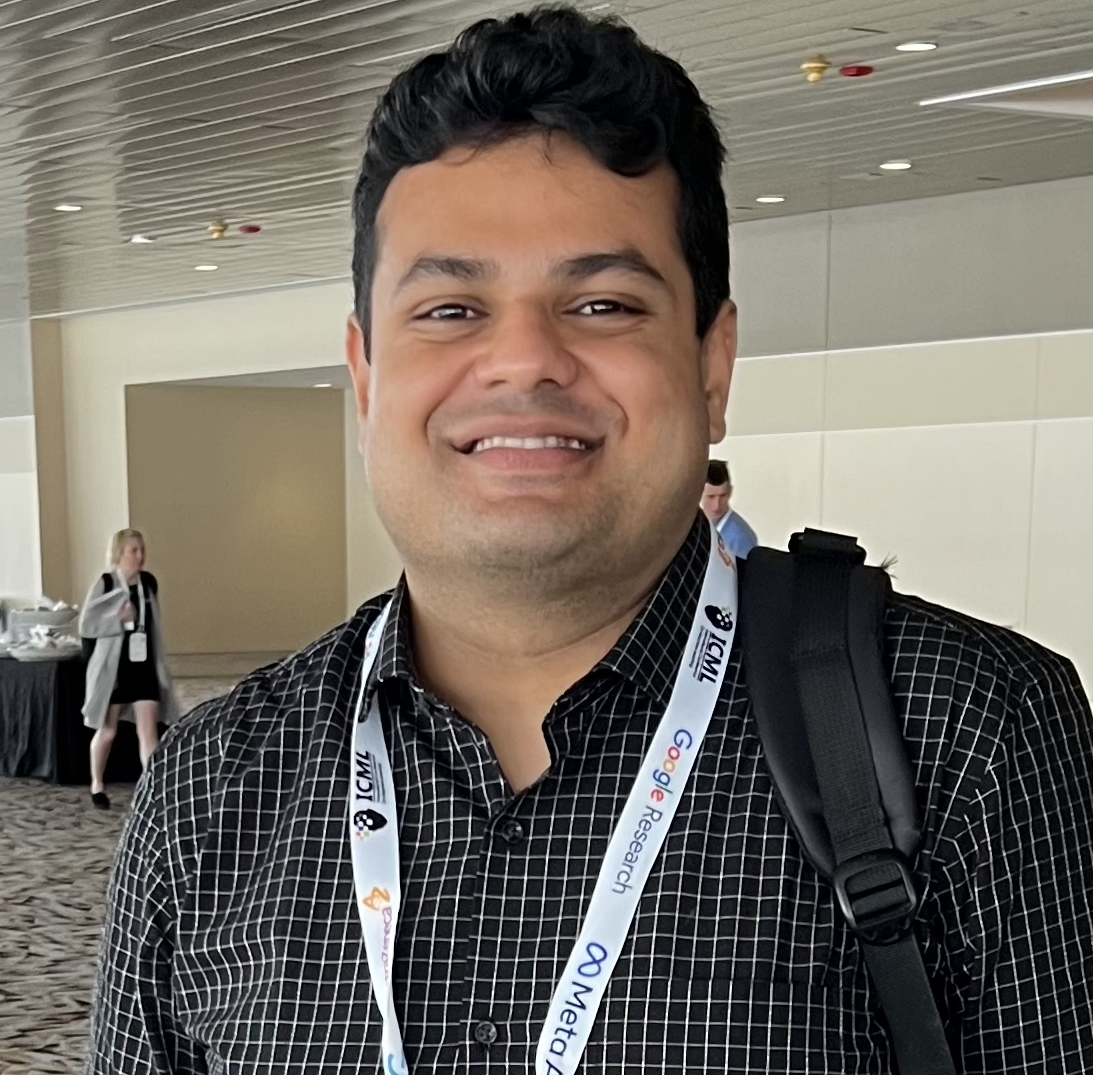
\includegraphics[width=0.5\linewidth]{img/Lecture0/Mohit_2024.png}}
\end{center}
\noindent\href{https://sites.google.com/view/mohit-prabhushankar}{Mohit Prabhushankar} received his Ph.D. degree in electrical engineering from the Georgia Institute of Technology (Georgia Tech) in 2021. He is currently a Postdoctoral Research Fellow and Instructor of Record in the School of Electrical and Computer Engineering at Georgia Tech in the Omni Lab for Intelligent Visual Engineering and Science (OLIVES). He is working in the fields of image processing, machine learning, active learning, healthcare, and robust and explainable AI. He is the recipient of the Best Paper award at ICIP 2019, Top Viewed Special Session Paper Award at ICIP 2020, and Best Paper runner-up award at BigData’24. He is the recipient of the ECE Outstanding Graduate Teaching Award, the CSIP Research award, and of the Roger P Webb ECE GRA Excellence award in 2022 and the Research Excellence Award in 2025. He has delivered short courses and tutorials at IEEE IV'23, ICIP'23, BigData'23, WACV'24, AAAI'24, CVPR'24, ICME'24, MIPR'24., WACV'25, and AAAI'25. 

\section{Disclaimer}
All content of this book are part of ECE 4252/6252 course at Georgia Institute of Technology. Any re-use or distribution is not permitted without pre-approved permission. All these materials belong to, created by, and copyrighted for Ghassan AlRegib and Mohit Prabhushankar, Georgia Tech, 2021-2028.

\section{Contributors}

Contributors to the course and slides include Dr. Ahmad Mustafa, Dr. Motaz Alfarraj, Dr. Ashraf Alattar, and Dr. Chen Zhou.

Teaching Assistants with remarkable contributions include: Kuo-Wei Lai, Shiva Mahato, Michael Zhou, and Yogita Choudhary.

\section{License} 

These lecture notes are licensed under the \href{https://creativecommons.org/licenses/by-nc-sa/4.0/}{Creative Commons Attribution-NonCommercial-ShareAlike 4.0} International License.

\end{document}